\externaldocument{main.tex}
As laid out in \ref{subsec:why-use-electron}, Browsers are significantly more powerful than ever. 
The \emph{browser wars} of the mid-to-late nineties started with Microsoft and Netscape outdoing each other with
new features, faster and overall better browsers leading to significant leaps in browser technology. \parencite{mozilla2021}\paragraph{}
Furthermore, internet access is more widespread than ever.
In the United States, the number of internet users rose from 229,91 million in 2010 to 302,28 million in 2021,
which constitutes a 31\% increase.\par
\begin{figure}[H]
    \label{fig:num-of-internet-users}
    \caption{Number of internet users from 2010 to 2025. \parencite{statista2021}}
    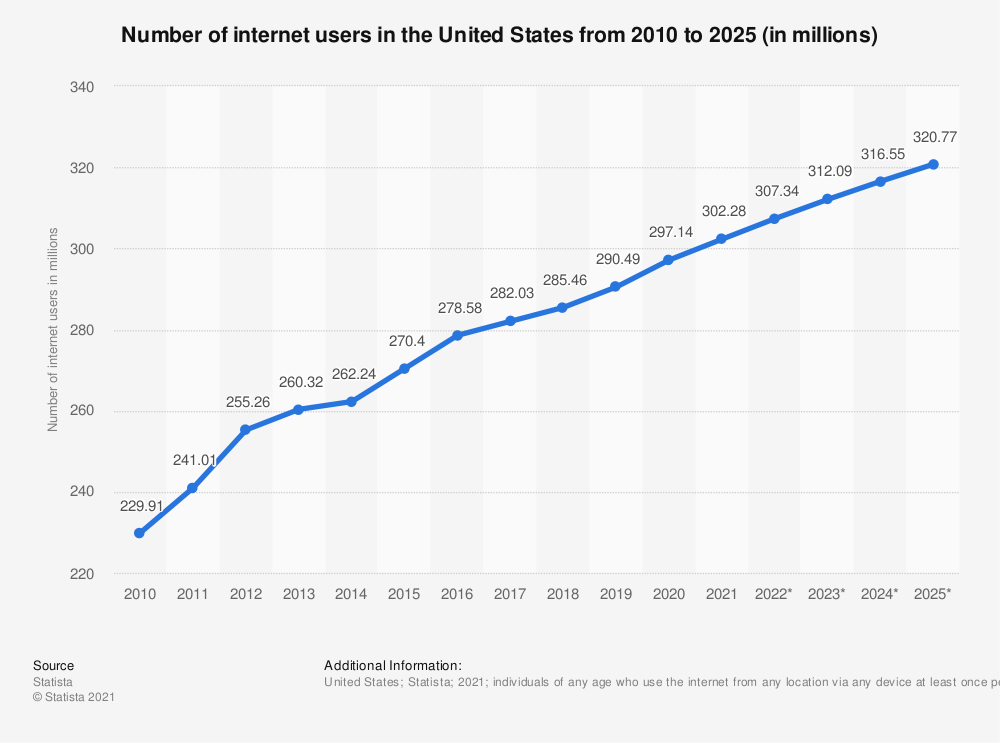
\includegraphics[width=0.8\textwidth]{number-of-internet-users}
\end{figure}
And not have the number of internet users risen over the past 11 years, the average connection speed increased as well
over the same time period:

and faster, and the number
of robust frameworks for web development (be it front-end or back-end), make creating a complex web application easier
than ever before. \parencite{akamai2017, statista2021}
Additionally, SaaS can be developed more easily than native desktop applications because in a web environment there is no
need to port to all the different platforms one wants to support. 
Moreover the software provider has strict control over when updates occur in contrast to users having to manually update their 
desktop applications and should bugs occur, developers can reproduce said bugs much more easily with real-world data. \parencite{jacobs2005}\paragraph{}
However, web applications come with their disadvantages. Due to browser security access to a user's file system is not possible, for example.
Furthermore, some users may have a personal preference towards traditional desktop applications. 
